%%%% ijcai19.tex

\typeout{Aggregation for open-ended task}

% These are the instructions for authors for IJCAI-19.

\documentclass{article}
\pdfpagewidth=8.5in
\pdfpageheight=11in
% The file ijcai19.sty is NOT the same than previous years'
\usepackage{ijcai19}

% Use the postscript times font!
\usepackage{times}
\usepackage{soul}
\usepackage{url}
\usepackage[hidelinks]{hyperref}
\usepackage[utf8]{inputenc}
\usepackage[small]{caption}
\usepackage{graphicx}
\usepackage{subcaption}
\usepackage{amsmath}
\usepackage{booktabs}
\usepackage{algorithm}
\usepackage{algorithmic}
\usepackage{amsmath, amsthm, amssymb}
\usepackage{bbm}
\urlstyle{same}
\usepackage{pgfplots, pgfplotstable}
\usepackage[T1]{fontenc}
\usepackage{colortbl}
\usepackage{amsmath}
\usepackage{url}
\usepackage{xspace}
\usepackage{tikz}
\usetikzlibrary{bayesnet}
\newcommand{\argmax}[1]{\underset{#1}{\operatorname{arg}\,\operatorname{max}}\;}
\usepackage[algo2e,titlenotnumbered,boxed,ruled,vlined,linesnumbered]{algorithm2e}
\usepackage{stackengine}
\def\delequal{\mathrel{\ensurestackMath{\stackon[1pt]{=}{\scriptstyle\Delta}}}}

\newcommand{\sys}{OpenCrowd\xspace}


\newcommand{\mkh}[1]{\textcolor{red}{(*** MK: #1 ***)}}
\newcommand{\iar}[1]{\textcolor{blue}{(*** @Ines: #1 ***)}}
\newcommand{\jie}[1]{\textcolor{green}{(*** @Jie: #1 ***)}}

% the following package is optional:
%\usepackage{latexsym} 
\title{\sys: Finding Social Influencers using Open-Ended Answer Aggregation}

% Single author syntax
\author{
Paper ID: 4876
%    XI Lab
%    \affiliations
%    University of Fribourg, Switzerland\emails
%    firstname.lastname@unifr.ch
}

% Multiple author syntax (remove the single-author syntax above and the \iffalse ... \fi here)
% Check the ijcai19-multiauthor.tex file for detailed instructions
\iffalse
\author{
First Author$^1$
\and
Second Author$^2$\and
Third Author$^{2,3}$\And
Fourth Author$^4$
\affiliations
$^1$First Affiliation\\
$^2$Second Affiliation\\
$^3$Third Affiliation\\
$^4$Fourth Affiliation
\emails
\{first, second\}@example.com,
third@other.example.com,
fourth@example.com
}
\fi

\begin{document}

\maketitle

\begin{abstract}
Finding social influencers is a fundamental task in many online applications, ranging from brand marketing to opinion mining. Existing methods are mainly based on supervised learning techniques, whose performance is heavily limited by the availability of expert labels (often limited). Unlike experts, the crowd possesses a more broad knowledge -- on an aggregated level -- of influencers in many domains, such as fashion and fitness. Individual crowd workers, however, only possess fragmented knowledge that is often of low-quality. In this paper, we introduce \sys, a new Expectation-Maximization (EM) learning framework, to effectively find social influencers by asking the crowd in the form of open-ended questions. In particular, we derive an efficient variational inference algorithm to infer the true influencers by aggregating fragmented crowd contributions while learning the reliability of individual crowd workers. Experimental results on real-world datasets show that our approach substantially improves the state of the art.
\end{abstract}





\label{sec:intro}
%%%%%%%%%%%%%%%%%%%%%%%%%
\section{Introduction}
%%%%%%%%%%%%%%%%%%%%%%%%%

Social influence is an important mechanism that regulates the dynamics of social networks. Social influencers are users who regularly produce authoritative or novel content on specific topics and who can reach a wide number of followers. Finding social influencers has become a fundamental task in many online applications, ranging from brand marketing
~\cite{bond201261,richardson2002mining,van2007new} to opinion mining \cite{pang2008opinion,li2012mining}, expert finding for question 
answering~\cite{riahi2012finding}, misinformation propagation~\cite{DBLP:conf/icde/SongHL17} or task execution \pcm{rephrase this one, unclear what this means}~\cite{sun2014analyzing,miao2010generative}. 

The task of finding social influencers is, however, extremely challenging due to the subjectivity in perceiving social influence and the requirement for expert knowledge in determining the authenticity of user-generated content. Existing work mainly tackles the problem using supervised learning approaches that rely on a training set hand-labeled by domain experts \cite{Cheng2014,Lehmann2013,wei2016learning}. Such an approach can be viewed as a way of transferring expert knowledge to learning models through the training data. While models trained in this fashion are effective at finding social influencers who are similar to those in the training data, they are intrinsically limited by the availability of expert labels, which are typically very hard to gather and hence highly limited. As an example, our collaboration with a major fashion company reveals that an expert can only recognize no more than 200 fashion influencers on Twitter over a 3-week period of time. Finding social influencers is, therefore, a long and usually laborious process even for domain experts.

Compared to an individual expert, online crowds 
%-- as the \emph{direct influencee} in a social network -- 
possess as a whole a broader knowledge of social influencers in various domains, e.g., fashion, fitness, or information technology. Therefore, we advocate in this paper a human computation approach that crowdsources the task of finding social influencers in the form of open-ended question-answering. Specifically, we consider a task where the crowd is asked to name as many as possible social influencers in a predefined domain. By aggregating the answers from a large number of crowd workers, we can identify the identities (e.g., usernames on Twitter) of a large number of social influencers in a efficient and cost-effective manner. 

Despite its obvious benefit, aggregating open-ended answers from the crowd is however challenging: individual crowd workers may only possess fragmented knowledge that is of low-quality. While answer aggregation has been extensively studied in human computation \cite{dawid1979maximum,whitehill2009whose,ZhengLLSC17}, we note that existing methods are not applicable in our context of open-ended answers. Previous methods mainly consider classification problems, where crowd workers are asked to classify a existing, \emph{closed} pools of data instances into \emph{pre-defined classes}. While in our context, we consider an \emph{open} pool of answers that are \emph{all deemed relevant} by crowd workers. How to aggregate open-ended answers contributed by crowd workers with various knowledge levels therefore remains a key open research question.

To address this problem, we introduce \sys, a new probabilistic learning and inference framework based on Expectation Maximization (EM) for open-ended answers aggregation. Our framework models both the workers reliability and the quality of the answers as latent variables, and infers these variables in an iterative and mutually boosting manner through EM. A small number of labeled answers is used as the seed for starting the inference -- our framework can thus be viewed as an extension of ``learning from crowds''  \cite{raykar2010learning,yan2010modeling,tian2012learning} to the semi-supervised learning scenario. Given the different number of answers contributed by workers, we propose a Bayesian version of the framework and a variational inference algorithm that characterize the uncertainty in inferring worker reliability, which improves both the robustness of the framework as well as its interpretability. 

In summary, we make the following key contributions:
\begin{itemize}
\item We formally define the problem of finding social influencers through open-ended answers aggregation;
\item We introduce a new EM-based learning and inference framework for open-ended answers aggregation; and
\item We present a Bayesian version of the framework together with an efficient variational inference algorithm for parameter estimation. 
\end{itemize}

To the best of our knowledge, we are the first to adopt an open-ended answer aggregation approach for finding social influencers. Our extensive empirical evaluation on two domains -- fashion and information technology -- demonstrates that \sys substantially improves the state of the art by \pcm{fill in missing numbers} XXX\% accuracy and XXX\% AUC. 

\label{sec:problem}
%%%%%%%%%%%%%%%%%%%%%%%%%
\section{Problem Formulation}
%%%%%%%%%%%%%%%%%%%%%%%%%

In this section, we first introduce the notations used in the paper and then formally define the open-ended answers aggregation problem.

\smallskip
\noindent\textbf{Notations.} Throughout this paper, we use boldface lowercase letters to denote vectors and boldface uppercase letters to denote matrices. For an arbitrary matrix $\mathbf{M}$, we use $\mathbf{M}_{i,j}$ to denote the entry at the $i$-th row and $j$-th column. We use capital letters (e.g., $\mathcal{P}$) in calligraphic math font to denote sets.

We use $\mathcal{I}$ to denote the set of unique \emph{candidate} social influencers named by the crowd workers, and $\mathcal{J}$ to denote the set of workers. We use $\mathbf{A}_{i,j}=1$ to denote that the candidate influencer $i$ is an answer provided by worker $j$, and $\mathbf{A}_{i,j}=0$ otherwise. Note that $\mathbf{A}_{i,j}$ is a sparse matrix where only a small proportion of the entries are non-zero. 
For each candidate influencer $i \in \mathcal{I}$, we collect her social features, such as number of followers, number of tweets, and the content of her tweets, and denote the resulting feature vector by $\mathbf{x}_i$. For a subset of $\mathcal{I}$, denoted as $\mathcal{I_L} \subset \mathcal{I}$, we are given an expert label $y_i$ for each candidate influencer $i$ in this subset ($i\in \mathcal{LI}$). Note that we only have a relatively small number of candidate influencers with expert labels, namely, $|\mathcal{I_L}| \ll |\mathcal{I}|$. %and similarly, each worker $j \in \mathcal{J}$ has a feature vector $\mathbf{y}_j$. 


% Our goal is to find those candidate  in $\mathcal{I}$ that are of high-quality, denoted by $\mathcal{SI} \subset \mathcal{I}$. We use $z_i = 1$ to denote $i\in \mathcal{SI}$, and $z_i = 0$ otherwise.

With the given notations, we formally define the problem of open-ended answers aggregation as follows.

\smallskip
\noindent\textbf{Problem Definition.} Given a set of candidate social influencers $\mathcal{I}$, their social features $\mathbf{x}_i$ $(i \in \mathcal{I})$, and a set of workers $\mathcal{J}$ who collectively nominated $\mathcal{I}$, we aim at inferring true labels $z_i \in \{0,1\}$ for all candidate influencers by leveraging the answer matrix $\mathbf{A}$, as well as existing labels $y_i$ for the limited number of labeled candidate influencers $i\in \mathcal{I_L}$. 

\label{sec:method}
%%%%%%%%%%%%%%%%%%%%%%%%%
\section{The \sys Framework}
%%%%%%%%%%%%%%%%%%%%%%%%%

\sys is a probabilistic framework that aggregates open-ended answers while taking into account worker reliability. In this section, we first introduce how \sys models the open-ended question-answering process, and then introduce the Expectation Maximization method for learning the parameters. Subsequently, we present a Bayesian version of our framework with an efficient variational inference algorithm for characterizing the uncertainty of worker relability. 

\subsection{\sys as a Generative Model}
To infer the true label of a candidate social influencer, we adopt a Bayesian network to describe the open-ended question-answering process as a generative process. In this process, the true label of a candidate influencer follows a Bernoulli distribution:
%
\begin{equation}
    z_i \sim Ber(\theta_i), \theta_i  = \sigma (f^{\mathcal{W}_I}(\mathbf{x}_i)),
    \label{eq:dis_item}
\end{equation}
%
where $\theta_i$ is the parameter of the distribution predicted by the social features of the candidate influencer through a linear model or a neural network, denoted by $f$; $\mathcal{W}_I$ is the parameter of the model; $\sigma$ is the sigmoid function. Note that $\mathcal{W}_I$ is shared among all candidate influencers, thus amortizing the inference \cite{gershman2014amortized} by exploiting the similarity among candidate influencers. 


We then model worker reliability by $r_j \in [0,1]$ $(j\in \mathcal{J})$, where $r_j=1$ indicates the worker is fully reliable and $r_j=0$ indicates the worker is not reliable. We use the reliability of a worker to define the probability of her named candidate influencer being a true influencer:
%
\begin{equation}
    p(\mathbf{A}_{i,j} | z_i,  r_j) = r_j^{\mathbbm{1}[z_i=\mathbf{A}_{i,j}]} (1- r_j)^{\mathbbm{1}[z_i\ne \mathbf{A}_{i,j}]},
    \label{eq:item_worker}
\end{equation}
%
where $\mathbbm{1}(\cdot)$ is an indicator function. Note that the above equation considers a worker to be reliable if she does not name a candidate influencer who turns out not be a not real influencer. It is, however, likely that a worker does not name a candidate influencer $i$ simply because she did not think of $i$. That means that we can only partly treat the non-named candidate influencers as those the worker considers as non-influencers. It is, therefore, necessary to introduce negative sampling into the inference algorithm, which we introduce in Section~\ref{sec:em}. 

Worker reliability $r_j$ is so far assumed to be a fixed parameter. In practice, we would like to distinguish our \emph{confidence} in estimating the reliability of the workers providing different numbers of answers: we should be more confident in estimating the reliability of workers who provide 50 answers than those who only provide 5 answers. To quantify the confidence in our inference, we adopt a Bayesian treatment of $r_j$ by introducing a prior:
%
\begin{equation}
        r_j \sim Beta(A,B).
        \label{eq:rj_dist}
\end{equation}
%
The incorporation of confidence will make our framework more robust to overfitting, as we show in our experiments. 

The overall \sys framework is depicted in Figure~\ref{fig:graphical_model}. Model learning concerns parameter learning for $\mathcal{W}_I$ (and $r_j$ when modeled as a fixed parameter) and posterior inference for $z_i$ (and $r_j$ when modeled as a latent variable).  

\begin{figure}[htb] 
{
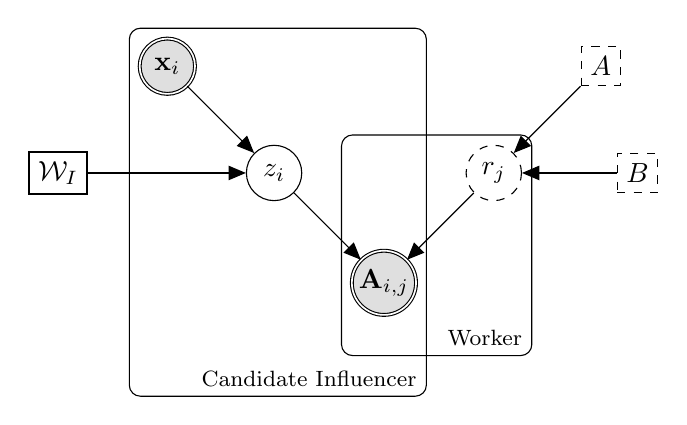
\begin{tikzpicture}

  % Define nodes
  \node[obs,double]          (a)   {$\mathbf{A}_{i,j}$}; %
  \node[latent, above left=1.2 of a]  (z)   {$z_i$}; %
  \node(rect) [latent, dashed, above right=1.2 of a]  (r)   {$r_j$};
  \node (rect)  [draw,dashed,minimum width=0.5cm,minimum height=0.5cm, above right=1.2 of r] (alpha){$A$};
  \node (rect)  [draw,dashed,minimum width=0.5cm,minimum height=0.5cm, right=1.2 of r] (beta){$B$};


  \node(rect)  [draw,thick,minimum width=0.5cm,minimum height=0.5cm, left=2 of z] (w) {$\mathcal{W}_I$} ; 
  \node[obs,double, above left=1.2 of z]  (x) {$\mathbf{x}_i$} ; %


  % Factors
  \edge {alpha,beta} {r} ;
  \edge {w, x} {z} ;
  \edge {z,r} {a} ;

  \plate {yx} {(a)(r)} {Worker} ;
  \plate {} {(a)(z) (x) (yx.north west)(yx.south west)} {Candidate Influencer} ;

\end{tikzpicture}
}
\caption{Graphical model of \sys. Double (greyed) circles represent observed variables, while single circles represent latent variables.  Squares represent model parameters. We note that worker reliability $r_j$ can either be a fixed parameter or a latent variable (thus, it is denoted by a dashed circle in the figure). Edges represent conditional relationship in answer generation.}
\label{fig:graphical_model}
\end{figure}


\subsection{Expectation Maximization for \sys} 
\label{sec:em}
For model learning, we first consider the case when worker reliability is modeled as a fixed parameter. Due to the latent variable $z_i$, we use Expectation Maximization (EM) \cite{dempster1977maximum}. Note that the EM method introduced below also serves as the basis for our variational inference method for the case when worker reliability is modeled as a latent variable. The EM method iteratively takes 1) the E-step to infer the posterior distribution over the true label $z_i$ ($i\in \mathcal{I}$) given the current estimates of model parameters, and 2) the M-step to learn the parameter $\mathbf{W}_I$ and $r_j$ ($j\in \mathcal{J}$) given the newly inferred latent variable.

For each worker $j\in \mathcal{J}$, we consider all candidate influencers named by her, and a random sample of candidate influencers she does not name -- obtained by negative sampling, as relevant candidate influencers in estimating her reliability. We denote such worker-relevant candidate influencers as $\mathcal{I}_j$; similarly, for each candidate influencer $i$, we denote all relevant workers, including those workers who do not name $i$ yet $i$ \pcm{? I couldn't understand this} is considered relevant by negative sampling, as $\mathcal{J}_i$.

\smallskip
\noindent\textbf{E-step.} We first denote $\mathbf{A}_{i,\mathcal{J}_i}$ as all relevant answers to candidate influencer $i$, i.e., $\mathbf{A}_{i,\mathcal{J}_i} = \{\mathbf{A}_{i,j}|j \in \mathcal{J}_i\}$. The E-step then infers the true label of a candidate influencer $i$ as follows:
%
\begin{align}
    p(z_i) & \delequal p(z_i|\mathbf{A}_{i,\mathcal{J}_i},r_{j},x_i,\mathcal{W}_I) \nonumber\\
        &\propto p(\mathbf{A}_{i,\mathcal{J}_i}|z_i,r_j)\times p(z_i|x_i,\mathcal{W}_I) \label{eq:dist_cond}\\
        &=\prod_{j \in \mathcal{J}_i} p(\mathbf{A}_{i,j}|z_i,r_{j})\times p(z_i|x_i,\mathcal{W}_I). \nonumber    
\end{align}
%
The inference of $z_i$ is therefore determined by both the reliability of the relevant workers' answers and the social features of the candidate influencer $i$. Note that $p(\mathbf{A}_{i,j}|z_i,r_{j})$ is defined by Equation~\ref{eq:item_worker} and $p(z_i|x_i,\mathcal{W}_I)$ is defined by Equation~\ref{eq:dis_item}.

\smallskip
\noindent\textbf{M-step.}
Given the the true labels of candidate influencers inferred by the E-step, the M-step maximizes the following log-likelihood function to learn the parameters:
\begin{align}
   \mathcal{L} 
    &=\sum_{z_i}p(z_i)\log p(\mathbf{A}_{i,j},z_i|r_j,\mathbf{x}_i,\mathcal{W}_I)\nonumber\\
    &=\sum_{z_i}p(z_i)\log (p(\mathbf{A}_{i,j}| z_i , r_j) \times p(z_i |\mathbf{x}_i;\mathcal{W}_I)) \label{eq:likelihood_m}\\
    &=\underbrace{\sum_{z_i}p(z_i) \log p(\mathbf{A}_{i,j}| z_i , r_j)}_{\mathcal{M}_1}
    +\underbrace{\sum_{z_i}p(z_i)\log p(z_i |\mathbf{x}_i;\mathcal{W}_I)}_{\mathcal{M}_2},
    \nonumber
\end{align}
where $p(z_i)$ is obtained by Equation~\ref{eq:dist_cond}. We observe that the M-step can be decomposed in two parts independent of each other. The first part, $\mathcal{M}_1$, can be solved via stochastic gradient ascent (SGA). The gradient of $r_j$ is given by:
%
\begin{equation}
    \frac{\partial \mathcal{M}_1}{\partial r_j}=\frac{p(\mathbf{A}_{i,j}=z_i)}{r_j}-\frac{p(\mathbf{A}_{i,j}\neq z_i)}{1-r_j}.
    \label{eq:grad_rj}
\end{equation}
%
The second part, $\mathcal{M}_2$, interestingly, is exactly the inverse of the cross-entropy between $p(z_i)$ and $p(z_i |\mathbf{x}_i;\mathcal{W}_I)$, which is widely used as the loss function for many classifiers. $\mathcal{M}_2$ can, therefore, be optimized using standard methods (e.g., back-propagation if a neural network is used by \sys).

\subsection{Variational Inference for \sys}
\label{sec:vi}

We now introduce our variational inference method for the Bayesian version of \sys, i.e., when worker reliability is modeled as a latent variable with a prior distribution. In this case, a closed form solution for the EM updates is no longer possible. We develop a meanfield variational approach to approximate the posterior distribution over all hidden variables given the data, which in our model is $p(\mathbf{z},\mathbf{r} | \mathcal{D})$, where $\mathbf{z}$ and $\mathbf{r}$ are the latent true labels for all candidate influencers and for the reliability of all workers, respectively, and $\mathcal{D}$ is the observed data, i.e., $\{\mathbf{A}, \mathbf{x}_i\ (\forall i\in\mathcal{I}), y_i\ (\forall i\in \mathcal{LI})\}$. 

The main idea of variational inference \cite{tzikas2008variational} is to approximate $p(\mathbf{z},\mathbf{r} | \mathcal{D})$ by a variational distribution $q(\mathbf{z},\mathbf{r})$ and perform optimization to minimize the KL divergence between the two distributions. Meanfield variational inference allows for efficient optimization by assuming that $q(\mathbf{z},\mathbf{r})$ factorizes over the latent variables:
\begin{equation}
    q(\mathbf{z},\mathbf{r})=\prod_{i} q(z_i) \prod_j q(r_j).
    \label{eq:dist_fact}
\end{equation}
%
We further assume the forms of the factor functions:
\begin{align}
    q(z_i)=Ber(\phi_i), q(r_j)=Beta(\alpha_j,\beta_j),
\end{align}
%
where $\phi_i$, $\alpha_j$ and $\beta_j$ are variational parameters used to perform optimization to minimize the KL-divergence. This optimization problem can be solved via coordinate ascent \cite{blei2017variational}: updating one factor while keeping all others fixed and iterating until convergence. In the following, we derive the update equations for the latent variables $z_i$ ($i\in\mathcal{I}$) and $r_j$ ($j\in\mathcal{J}$).

\smallskip
\noindent\textbf{Updating $z_i$.} For $z_i$, we have:
%
\begin{equation}
q(z_i)    \propto \prod_{j \in \mathcal{J}_{i}} \exp{\{\mathbb{E}_{q(r_j)}[\log (P(\mathbf{A}_{i,j}|z_i,r_j))]\}}   \times P(z_i|x_i, \mathcal{W}_I). \\
\end{equation}
%
We distinguish between two cases:
%
\begin{align}
    q(z_i=0)   &= \prod_{j \in \mathcal{J}_{i}} \exp{\{\mathbb{E}_{q(r_j)}[\log (1-r_j)]\}}\times (1-\theta_i) \nonumber, \\
    q(z_i=1)   &= \prod_{j \in \mathcal{J}_{i}} \exp{\{\mathbb{E}_{q(r_j)}[\log (r_j)]\}}\times \theta_i .
\label{eq:q_two_poss}                
\end{align}
%
The expectations can be evaluated as follows:
\begin{align}
    \mathbb{E}_{q(r_j)}[\log (1-r_j)]&= \Psi(\beta_j)-\Psi(\alpha_j+\beta_j), \nonumber \\
    \mathbb{E}_{q(r_j)}[\log (r_j)]&= \Psi(\alpha_j)-\Psi(\alpha_j+\beta_j),
    \label{eq:expect}
\end{align}
where $\Psi(\cdot)$ is the Digamma function. Therefore, the update equation for $z_i$ can be simplified as:
\begin{align}
    q(z_i=0)   &\propto \prod_{j \in \mathcal{J}_{i}} \exp{\{\Psi(\beta_j)-\Psi(\alpha_j+\beta_j)\}}\times (1-\theta_i), \nonumber \\  
     q(z_i=1)    &\propto \prod_{j \in \mathcal{J}_{i}} \exp{\{ \Psi(\alpha_j)-\Psi(\alpha_j+\beta_j)\}}\times \theta_i  .
     \label{eq:qzi}
\end{align}

\smallskip
\noindent\textbf{Updating $r_j$.}  For $r_j$, we have:
%
\begin{equation}
    q(r_j) \propto \prod_{i \in \mathcal{I}_j} \exp{\{\mathbb{E}_{q(z_i)}[\log{P(\mathbf{A}_{i,j}|r_j,z_i)}]\}} \times   {P(r_j)}
\end{equation}
%
where $P(r_j)$ is the variational $r_j$ distribution from last iteration. The expectation can be evaluated as follows:
%
\begin{align}  
& \exp{\{\mathbb{E}_{q(z_i)}[\log{P(\mathbf{A}_{i,j}|r_j,z_i)}]\}} = \nonumber \\
& 
\left\{  
    \begin{array}{lr}
        r_j^{\theta_i}  \times (1-r_j)^{(1 - \theta_i)}, &  \text{if\ } \mathbf{A}_{i,j}=1\\  
        r_j^{(1 - \theta_i)}  \times (1-r_j)^{\theta_i}, &  \text{if\ } \mathbf{A}_{i,j}=0   
    \end{array}  
\right.  
\end{align}
%
Therefore, $r_j$ can be efficiently inferred as follow:
%
\begin{align}  
& q(r_j)  \propto \nonumber \\
& 
\left\{  
    \begin{array}{lr}
        Beta(\alpha_j+\sum_{i\in \mathcal{I}_j}  \theta_i,\beta_j+ \sum_{i\in \mathcal{I}_j} (1 - \theta_i) ), &  \text{if\ } \mathbf{A}_{i,j}=1\\  
        Beta(\alpha_j+\sum_{i\in \mathcal{I}_j} (1 - \theta_i),\beta_j+ \sum_{i\in \mathcal{I}_j} \theta_i), &  \text{if\ } \mathbf{A}_{i,j}=0   
    \end{array}  
\right.  
\label{eq:qrj}
\end{align}



The update rules described above play the role of the E-step in a variational EM approach. 
The M-step for learning $\mathbf{W}_I$ can be performed in a similar manner as in the previous section. The overall coordinate ascent algorithm is presented in Algorithm~\ref{alg:vi-algo}. It iterates over the E-step and M-step until the evidence lower bound (ELBO) \cite{blei2017variational} -- equivalent to the KL-divergence as the optimization objective yet easily computable -- converges. We note that this algorithm has a similar computational complexity as the normal EM method: both Equations~\ref{eq:qzi} and \ref{eq:qrj} can be efficiently computed; and $\mathbf{W}_I$ can be efficiently updated in an incremental manner, i.e., it can learn for a few more epochs starting from the parameter learned in the previous iteration.

\begin{algorithm2e}
    \SetKwInOut{Input}{Input}
    \SetKwInOut{Output}{Output}
    \SetKwInOut{Initialize}{Initialize}
    \Input{$\mathbf{A}, \mathbf{x}_i\ (\forall i\in\mathcal{I}), y_i\ (\forall i\in \mathcal{LI})$}
    \Output{Variational distributions: $q(z_i)$ ($i\in \mathcal{I}$) and $q(r_j)$ ($j\in \mathcal{J}$)}
    \Initialize {Variational parameters: $\theta_i$, $\alpha_j=A$, $\beta_j=B$; parameter of the influencer predictor ($f$): $\mathbf{W}_I$}
    \While{the ELBO has not converged}{
    E-step:\\
        \For {$i \in \mathcal{I}$}
        {
                update $q(z_i)$ by Equation~\ref{eq:qzi}\;
        } 
        \For {$j \in \mathcal{J}$}
        {
                update $q(r_j)$ by Equation~\ref{eq:qrj}\;
        }
       M-step: \\
        \For {$i \in \mathcal{I}$}
        {
         Update $\mathcal{W}_I$ via standard gradient descent\;
       } 
    }
    \caption{Coordinate Ascent Variational Inference}
    \label{alg:vi-algo}
\end{algorithm2e}

\label{sec:result}
%%%%%%%%%%%%%%%%%%%%%%%%%
\section{Experiments and Results}

\subsection{Experimental Setup}

\noindent\textbf{Datasets.} We consider the problem of finding social influencers in two domains: fashion and information technology (InfoTech). For both domains, we publish question-answering tasks in Figure Eight\footnote{\url{https://www.figure-eight.com}} and collect crowd workers' answers. Key statistics of these datasets are reported in Table~\ref{tab:datasets}. For both datasets, we randomly select 40\% of the candidate influencers and ask domain experts to label them. Our initial analysis reveals that 30.64\% and 32.78\%  of the crowd answers are true influencers for Fashion and InfoTech, respectively. Considering the relatively large number of crowd answers collected in a short period of time ($<$10 hours for both Fashion and InfoTech), this result validates our assumption that crowdsourced open-ended question-answering provides an efficient way for finding social influncers. Moreover, the high sparsity of the answer matrices (Table~\ref{tab:datasets}) and the fact that the majority of the answers being incorrect verify the necessity of open-ended answers aggregation that takes into account worker reliability.

\begin{table}[!ht]
%\small
\centering \caption{Descriptive statistics of the
datasets.}\label{tab:datasets}
%\vspace{-0.05in}
\addtolength{\tabcolsep}{-1mm}
\begin{tabular}{lcccc}
\toprule
    Datasets & \textbf{\#Cand. Infl.} & \textbf{\#Workers} & \textbf{\#Answers} & \textbf{Sparsity}   \\\midrule
    Fashion & 890 & 250 & 1416  & 99.36\% \\
    InfoTech & 1057 & 200 &1643 & 99.22\% \\
\bottomrule
\end{tabular}
% \vspace{-0.1in}
\end{table}

\begin{table*}[t]
\centering
\caption{Performance (accuracy and AUC) of comparsion methods on the two datasets with supervision degree $s\_deg$ from 50\% to 90\%. The best performance is highlighted in bold; and the second best performance is marked by `*' for accuracy and by `+' for AUC.}\label{tab:comparision} 
\begin{tabular}{ll|ccccc|ccccc}
\toprule
\multirow{2}{*}{\textbf{Method}}  &   \multirow{2}{*}{\textbf{Metric}}  & \multicolumn{5}{|c|}{\textbf{Fashion}}      & \multicolumn{5}{c}{\textbf{InfoTech}} \jie{to update} \\ \cline{3-12}
 & &   50\%           & 60\%           & 70\%           & 80\%           & 90\%           & 50\%           & 60\%           & 70\%           & 80\%           & 90\%           \\ \midrule
\multirow{2}{*}{DS}          & Accuracy     & 0.689          & 0.716*         & 0.703          & 0.688          & 0.711*         & 0.662          & 0.660          & 0.626          & 0.641          & 0.536          \\ % \cline{2-12} 
                             & AUC   & 0.191          & 0.169          & 0.242+          & 0.244          & 0.263          & 0.174          & 0.203*         & 0.222*         & 0.255          & 0.272          \\ \hline
\multirow{2}{*}{GLAD}        & Accuracy     & 0.697          & 0.716*         & 0.724          & 0.700          & 0.688          & 0.669*         & 0.667          & 0.637          & 0.672          & 0.595          \\ %\cline{2-12} 
                             & AUC   & 0.183          & 0.189          & 0.229          & 0.224          & 0.263          & 0.150          & 0.186          & 0.138          & 0.219          & 0.307*         \\ \hline
ZenCrowd                           & Accuracy     & 0.701          & 0.686          & 0.733* & 0.702*         & 0.688          & 0.651          & 0.674*         & \textbf{0.664} & \textbf{0.683} & 0.627*         \\ %\cline{2-12} 
                             & AUC   & 0.157          & 0.175          & 0.203         & 0.239          & 0.287+         & 0.146          & 0.198          & 0.212          & 0.246          & 0.234          \\ \hline
\multirow{2}{*}{LFC}         & Accuracy     & 0.721*         & 0.694          & 0.718          & 0.691          & 0.755          & 0.653          & 0.627          & 0.643          & 0.616          & 0.636          \\ %\cline{2-12} 
                             & AUC   & 0.203+         & 0.203+         & 0.225          & 0.264+         & 0.277          & 0.189*         & 0.192          & 0.215          & 0.276*         & 0.307*         \\ \hline
\multirow{2}{*}{OpenCrowd}   & Accuracy     & \textbf{0.751} & \textbf{0.740} & \textbf{0.733}         & \textbf{0.7694} & \textbf{0.889}  & \textbf{0.673} & \textbf{0.674} & 0.662*         & 0.672*         & \textbf{0.686} \\ % \cline{2-12} 
                             & auprc   & \textbf{0.304} & \textbf{0.350} & \textbf{0.350} & \textbf{0.452} & \textbf{0.495} & \textbf{0.207} & \textbf{0.213} & \textbf{0.267} & \textbf{0.300} & \textbf{0.333} \\ \bottomrule
\end{tabular}
 \label{sec:compres}  
\end{table*}

\smallskip
\noindent\textbf{Comparison Methods.} Due to the lack of existing open-ended answers aggregation methods, we compare with the following state-of-the-art closed-pool answers aggregation methods: 1) ZenCrowd \cite{demartini2012zencrowd}, EM method that estimates worker reliability as a model parameter; 2) Dawid-Skene \cite{dawid1979maximum}, EM method that learns worker reliability as a confusion matrix; 3) GLAD \cite{whitehill2009whose}, EM method that simutaneously learn worker reliability and task difficulty; and 4) LFC \cite{raykar2010learning}, EM method 
that incorporate priors in modeling worker reliability. To apply these methods to our problem, we use negative sampling to simulate workers' answers of non-influencers; we empirically find the optimal sampling rates for each comparison method. 

To investigate the benefit of modeling worker reliability as compared to feature-based methods, we compare logistic regression (LR) and multi-layer perceptron (MLP) with two variants of our framework: 1) \sys-EM: \sys that aggregates workers' answers however models worker reliability as a fixed paramter; and 2) \sys, the Bayesian version that models worker reliability as a latent variable.




\smallskip
\noindent\textbf{Parameter Settings.} The parameters of our framework and those for model training are empirically set. We search for the best model architecture for MLP, and the predictor $f$ in \sys-EM and \sys, with 0, 1, and 2 hidden layers, and apply a grid search in \{64, 128, 256, 512, 1024\} for the dimension of the hidden layers. In model training, we select learning rates from \{0.0001, 0.001, 0.01, 0.1, 1\} for the learning of $\mathbf{W}_I$ in all variants of our framework, as well as for the learning of $r_j$ in \sys-EM. To investigate the impact of negative sampling, we experiment with sampling rate ($s\_rate$) from \{0, 1, 5, 10, 20, 50, 100\} where $s\_rate=5$ indicates that for each worker, the negative samples is five times the size of the candidate influencers named by each worker. 

\smallskip
\noindent\textbf{Evaluation Protocols.} We split the labeled subset of candidate influencers into training, validation, and test sets. \sys is trained on the answers and the training set, tuned on the valiation set and evaluated on the test set. To investigate the impact of the degree of supervision ($s\_deg$) on \sys performance, we split the labeled subset by $s\_deg\in \{50\%, 60\%, 70\%, 80\%, 90\%\}$, where $s\_deg = 60\%$ means that 60\% of the labeled subset is used for training, and the rest for validation and test with equal split. We use accuracy and area under the precision-recall curve (AUC) to measure the performance. Higher values of accuracy and AUC indicate better performance.



\subsection{Comparative Results}
Table~\ref{sec:compres} summarizes the performance of the compared answers aggregation methods on the two datasets with different supervision degree. Several interesting findings are observed.

First, we observe that ZenCrowd generally outperforms DS and GLAD. Recall that ZenCrowd is less expressive compared to DS and GLAD, as it only models worker reliability as a parameter. In comparison, DS models worker reliability as a confusion matrix, and GLAD futher models the task difficulty (in our context the ambiguity of a candidate influencer being the true influencer). The superior performance of ZenCrowd to that of DS and GLAD indicates that in our context, more expressive models do not necessary lead to higher performance. This is likely due to the high sparsity of worker-answer matrices (Table~\ref{tab:datasets}) that can easily lead to overfitting.

Second, we observe that methods that model worker reliability as a latent variable with a prior distribution, namely LFC and our framework \sys, outperform the other methods. Such a result verifies the necessity of modeling worker reliability as a latent variable, as it helps to account for the confidence of estimating model parameters. This is particularly important to improve model robustness for sparse datasets as in our case. We  will give more results on this point in Section~\ref{sec:selfres}.

Most importantly, our framework \sys achieves the best performance among all answers aggregation methods under comparsion: \sys improves the state of the art by \jie{add numbers} XX\% accuracy and XX\% AUC on Fashion, and by XX\% accuracy and XX\% AUC on InfoTech. The big improvements clearly demonstrate the effectiveness of our framework in open-ended answers aggregation. 



\smallskip
\noindent\textbf{Impacts of Supervision Degree.} The supervision degree $s\_deg$ controls the amount of observed labels in model training. We observe that the performance of our framework increases along with the increase of $s\_deg$, as measured by both accuracy and AUC. This is natural as more labeled data provides more information in discriminating influencers from non influencers. Such a pattern, however, is not observed for the other methods that we compare to. This is likely due to the fact that the other methods do not take advantage of the social features, which are useful as they serve as means to propagate the labels to non-labeled candidate influencers. These results, therefore, suggest that \sys is better at utilizing existing labels for answers aggregation. 

\subsection{Results of \sys}
\label{sec:selfres}

\noindent\textbf{Results of \sys Variants.}
The comparison between \sys variants against feature-based methods is shown in Figure \ref{fig:variants}. \sys-EM outperforms both LR and MLP by 13.05\% and XX\% accuracy and by 3.435\% and XX\% AUC, respectively. These results clearly show the importance of considering worker reliability in aggregating workers' answers. Among the two variants, \sys performs outperforms \sys-EM by 1.7\% accuracy and XX\% AUC. This result indicates that modeling the worker reliability as a latent variable with a prior distribution not only makes the model more robust, but also improves the aggregation performance in terms of accuracy and AUC. 
\begin{figure}[htb]
\begin{subfigure}[t]{0.47\columnwidth}
        \centering
    \pgfplotstableread[row sep=\\,col sep=&]{
       cases & LR & MLP & EM & VEM \\
       Fashion     &0.604166667  & 0.7006  & 0.7333 &0.7555  \\
       InfoTech    & 0.511 & 0.6  & 0.641&0.647 \\
    }\mydata

    \begin{tikzpicture}[scale=0.5]
    \begin{axis}[
    ybar,
    bar width=.55cm,
    width=2\textwidth,
    height=1.5\textwidth,
    legend style={at={(1.2,1.2)},
       anchor=north,legend columns= 4, font = \LARGE},
    symbolic x coords={Fashion, InfoTech},
    xtick=data,
    enlarge x limits=0.3,
    ymin=0.4,ymax=0.80,
    ylabel={Accuracy},
    yticklabel style = {font=\huge,xshift=0.5ex},
    xticklabel style = {font=\huge,yshift=0.5ex},
    ylabel style ={font = \huge},
    ymajorgrids=true
    ]
    \addplot[draw=gray,fill=gray!40!white, thick] table[x=cases,y=LR]{\mydata};
    \addplot[draw=blue,fill=blue!40!white] table[x=cases,y=MLP]{\mydata};
    \addplot[draw=black,fill=black!50!white, thick] table[x=cases,y=EM]{\mydata};
    \addplot[draw=red,fill=red!40!white, thick] table[x=cases,y=VEM]{\mydata};
    \legend{LR, MLP, \sys-EM, \sys}
    \end{axis}
    \end{tikzpicture}
    \vspace{-0.15in}
        \caption{Accuracy\label{fig:acc}} 
    \end{subfigure}% 
  \hfill \hskip -2.5ex %
    	\begin{subfigure}[t]{0.47\columnwidth}
        \centering
  \centering
    \pgfplotstableread[row sep=\\,col sep=&]{
       cases & LR & MLP & EM & VEM \\
       Fashion     &0.235142445  & 0.2154  &0.277139619 &0.42670444  \\
       InfoTech   &0.18673464  & 0.2154  & 0.2134 &0.2137 \\
    }\mydata

    \begin{tikzpicture}[scale=0.5]
    \begin{axis}[
    ybar,
    bar width=.55cm,
    width=2\textwidth,
    height=1.5\textwidth,
    legend style={at={(0.67,1.2)},
       anchor=north,legend columns= 4, font = \LARGE},
    symbolic x coords={Fashion, InfoTech},
    xtick=data,
    enlarge x limits=0.3,
    ymin=0.1,ymax=0.5,
    ylabel={AUCPR},
    yticklabel style = {font=\huge,xshift=0.5ex},
    xticklabel style = {font=\huge,yshift=0.5ex},
    ylabel style ={font = \huge},
    ymajorgrids=true
    ]
    \addplot[draw=gray,fill=gray!40!white, thick] table[x=cases,y=LR]{\mydata};
    \addplot[draw=blue,fill=blue!40!white] table[x=cases,y=MLP]{\mydata};
    \addplot[draw=black,fill=black!50!white, thick] table[x=cases,y=EM]{\mydata};
    \addplot[draw=red,fill=red!40!white, thick] table[x=cases,y=VEM]{\mydata};
    \legend{}
    \end{axis}
    \end{tikzpicture}
    \vspace{-0.15in}
        \caption{AUC\label{fig:AUC}} 
    \end{subfigure}% 
   \caption{Performance of our four variants.} \label{fig:variants}
\end{figure}

To quantitatively show the effect of modeling worker reliability as a latent variable, we depict in Figure~\ref{fig:XXX} \jie{to add} two examples of workers of similar reliability yet providing different number of answers. We observe that their reliability, as estimated by \sys-EM, are hardly distinguiable; however, \sys provides extra insight that the estimated reliability of the left worker is more trustable than that of the right worker.



\smallskip
\noindent\textbf{Impacts of Sampling Rate.}
The sampling rate $s\_rate$ controls the size of randomly sampled candidate influencers in estimating workers' reliability. The results are shown in Figure~\ref{fig:sys_perf_it}. We observe that, as the sampling rate varies from 0 to 100, the performance first increases then decreases. Such a result is consistent on both datasets, measured by both accuracy and AUC. The maximum performance is reached for $s\_rate= 10$ for Fashion and $s\_rate= 50$ for InfoTech, indicating that workers evaluation about the candidate influencers they do not name is more negative in InfoTech. Overal, the variation of the performance with different $s\_rate$ indicates the importance of selecting the optimal sampling rate. The similarity in performance variation across the two datasets demonstrates the robustness of \sys.

\begin{figure}[htb]\centering
	\begin{subfigure}[t]{0.47\columnwidth}
\begin{tikzpicture}[scale=0.5]
\begin{axis}[
    xlabel={Sampling Rate},
    ylabel={Accuracy},
    xmin=0, xmax=100,
    ymin=0.6, ymax=0.8,
    xtick={0,20,40,60,80,100},
    ytick={0.6,0.65,0.7,0.75,0.8},
       legend style={at={(1.15,1.2)},
       anchor=north,legend columns= 4, font = \LARGE},
    yticklabel style = {font=\huge,xshift=0.5ex},
    xticklabel style = {font=\huge,yshift=0.5ex},
    ylabel style ={font = \huge},
    xlabel style ={font = \huge},
    ymajorgrids=true,
    grid style=dashed,
    width=2\textwidth,
    height=1.5\textwidth
]
\addplot[
    color=blue,
    mark=square,
    ]
    coordinates 
 {
    (0,0.5861)
    (1,0.625)
    (5,0.715)
    (10,0.7027)
    (20,0.6986)
    (50,0.68888)
    (80,0.6805)
    (100,0.6944)
    };
   \addplot plot coordinates {
            (0,   0.625)
            (1,   0.6111)
            (5,  0.70138)
            (10, 0.75555)
            (20,  0.6805555)
            (50,  0.6805555)
             (80,  0.6805555)
             (100,  0.6805555)
        };   
\legend{\sys-EM, \sys}
\end{axis}
\end{tikzpicture}
    \vspace{-0.15in}
        \caption{Fashion - Accuracy\label{fig:acc_sr}} 
 \end{subfigure}
 \begin{subfigure}[t]{0.47\columnwidth}
\begin{tikzpicture}[scale=0.5]
\begin{axis}[
    xlabel={Sampling Rate},
    ylabel={AUC},
    xmin=0, xmax=100,
    ymin=0.2, ymax=0.4,
    xtick={0,20,40,60,80,100},
    ytick={0.2,0.25,0.3,0.35,0.4},
       legend style={at={(0.67,1.2)},
       anchor=north,legend columns= 4, font = \LARGE},
    yticklabel style = {font=\huge,xshift=0.5ex},
    xticklabel style = {font=\huge,yshift=0.5ex},
    ylabel style ={font = \huge},
    xlabel style ={font = \huge},
    ymajorgrids=true,
    grid style=dashed,
    width=2\textwidth,
    height=1.5\textwidth
]
\addplot[
    color=blue,
    mark=square,
    ]
    coordinates 
 {
(0,	0.2125)
(1,	0.23116	)
(5,	0.265159	)
(10,	0.25349)
(20,	0.349955)
(50,	0.342619	)
(80,	0.34914120	)
(100,	0.3486560	)
    };
   \addplot plot coordinates {
(0	,	0.3505)
(1	,	0.35039)
(5		,0.35033)
(10	,	0.35039)
(20	,0.350547)
(50	,0.35033)
(80	,	0.350392)
(100	,0.350547	)
        };   
\legend{}
\end{axis}
\end{tikzpicture}
    \vspace{-0.15in}
        \caption{Fashion - AUC\label{fig:AUC_sr}} 
 \end{subfigure}
   
	\begin{subfigure}[t]{0.47\columnwidth}
\begin{tikzpicture}[scale=0.5]
\begin{axis}[
    xlabel={Sampling Rate},
    ylabel={Accuracy},
    xmin=0, xmax=100,
    ymin=0.6, ymax=0.7,
    xtick={0,20,40,60,80,100},
    ytick={0.6,0.62,0.64,0.66,0.68,0.7},
       legend style={at={(0.67,1.2)},
       anchor=north,legend columns= 4, font = \LARGE},
    yticklabel style = {font=\huge,xshift=0.5ex},
    xticklabel style = {font=\huge,yshift=0.5ex},
    ylabel style ={font = \huge},
    xlabel style ={font = \huge},
    ymajorgrids=true,
    grid style=dashed,
    width=2\textwidth,
    height=1.5\textwidth
]
\addplot[
    color=blue,
    mark=square,
    ]
    coordinates 
 {
(0,	0.66941	)
(1,	0.68)	
(5,	0.6494)	
(10,	0.67411)	
(20,	0.67647)	
(50,	0.6811764)	
(80,	0.67411)	
(100, 0.6588)			
    };
   \addplot plot coordinates {
(0	,	0.62352)
(1	,	0.6341)
(5,	0.6423529)
(10	,	0.647058)
(20	,0.647058)
(50	,	0.647058)
(80	,	0.647058	)	
(100,	0.647058)
        };   
\legend{}
\end{axis}
\end{tikzpicture}
    \vspace{-0.15in}
        \caption{InfoTech - Accuracy\label{fig:acc_sr_it}} 
 \end{subfigure}
 \begin{subfigure}[t]{0.47\columnwidth}
\begin{tikzpicture}[scale=0.5]
\begin{axis}[
    xlabel={Sampling Rate},
    ylabel={AUC},
    xmin=0, xmax=100,
    ymin=0.1, ymax=0.4,
    xtick={0,20,40,60,80,100},
    ytick={0.1,0.15,0.2,0.25,0.3,0.35},
         legend style={at={(0.67,1.2)},
       anchor=north,legend columns= 4, font = \LARGE},
    yticklabel style = {font=\huge,xshift=0.5ex},
    xticklabel style = {font=\huge,yshift=0.5ex},
    ylabel style ={font = \huge},
    xlabel style ={font = \huge},
    ymajorgrids=true,
    grid style=dashed,
    width=2\textwidth,
    height=1.5\textwidth
]
\addplot[
    color=blue,
    mark=square,
    ]
    coordinates 
 {
(0	,0.2011	)
(1,	0.2027	)
(5,	0.2203	)
(10,	0.2134	)
(20,	0.2399	)
(50,	0.22034	)
(80,	0.1779664	)
(100,0.12080)	
    };
   \addplot plot coordinates {
(0,		0.19014)
(1	,	0.20389)
(5	,	0.19104)
(10,	0.2137225)
(20,	0.2112903)
(50,0.187791)
(80,	0.200248)
(100,	0.1940062)
        };   
\legend{}
\end{axis}
\end{tikzpicture}
 \caption{InfoTech - AUC\label{fig:AUC_sr_it}} 
 \end{subfigure}
   \caption{Performance of \sys with varying $s\_rate$.}\label{fig:sys_perf_it} 
\end{figure}


<<<<<<< HEAD
\subsection{Comparative Results}
Table \ref{tab:comparision} summarizes the performance of all comparison methods. We consider both Accuracy (acc)
and AUCPR to measure the effectiveness. Several interesting findings are observed as follows.
\begin{table*}[!h]
\centering
\begin{tabular}{|l|l|l|l|l|l|l|l|l|l|l|l|}
\hline
\multicolumn{2}{|l|}{Dataset}          & \multicolumn{5}{c|}{Fashion}                                                       & \multicolumn{5}{c|}{InfoTech}                                                            \\ \hline
\multicolumn{2}{|l|}{Supervision rate} & 50\%           & 60\%           & 70\%           & 80\%           & 90\%           & 50\%           & 60\%           & 70\%           & 80\%           & 90\%           \\ \hline
\multirow{2}{*}{DS}          & acc     & 0.689          & 0.716*         & 0.703          & 0.688          & 0.711*         & 0.662          & 0.660          & 0.626          & 0.641          & 0.536          \\ \cline{2-12} 
                             & AUC   & 0.191          & 0.169          & 0.242          & 0.244          & 0.263          & 0.174          & 0.203*         & 0.222*         & 0.255          & 0.272          \\ \hline
\multirow{2}{*}{GLAD}        & acc     & 0.697          & 0.716*         & 0.724          & 0.700          & 0.688          & 0.669*         & 0.667          & 0.637          & 0.672          & 0.595          \\ \cline{2-12} 
                             & AUC   & 0.183          & 0.189          & 0.229          & 0.224          & 0.263          & 0.150          & 0.186          & 0.138          & 0.219          & 0.307*         \\ \hline
ZC                           & acc     & 0.701          & 0.686          & 0.733* & 0.702*         & 0.688          & 0.651          & 0.674*         & \textbf{0.664} & \textbf{0.683} & 0.627*         \\ \cline{2-12} 
                             & AUC   & 0.157          & 0.175          & 0.203*         & 0.239          & 0.287*         & 0.146          & 0.198          & 0.212          & 0.246          & 0.234          \\ \hline
\multirow{2}{*}{LFC}         & acc     & 0.721*         & 0.694          & 0.718          & 0.691          & 0.755          & 0.653          & 0.627          & 0.643          & 0.616          & 0.636          \\ \cline{2-12} 
                             & AUC   & 0.203*         & 0.203*         & 0.225          & 0.264*         & 0.277          & 0.189*         & 0.192          & 0.215          & 0.276*         & 0.307*         \\ \hline
\multirow{2}{*}{OpenCrowd}   & acc     & \textbf{0.751} & \textbf{0.740} & \textbf{0.733}         & \textbf{0.769} & \textbf{0.889}  & \textbf{0.673} & \textbf{0.674} & 0.662*         & 0.672*         & \textbf{0.686} \\ \cline{2-12} 
                             & auprc   & \textbf{0.304} & \textbf{0.350} & \textbf{0.350} & \textbf{0.452} & \textbf{0.495} & \textbf{0.207} & \textbf{0.213} & \textbf{0.267} & \textbf{0.300} & \textbf{0.333} \\ \hline
\end{tabular}
   \caption{Performance in terms of Accuracy (acc) and AUC where best performance is highledted in bold and the second best performance is marked by `*' }\label{tab:comparision} 
\end{table*}
\label{sec:compres}

\smallskip
\noindent\textbf{Impacts of Supervision Degree.}
=======
>>>>>>> 5d1ad1530d6c64cab0e83234a32cd86bd164f089


\label{sec:related}
%%%%%%%%%%%%%%%%%%%%%%%%%
\section{Related Work}
%%%%%%%%%%%%%%%%%%%%%%%%%

In this section, we discuss relevant work on (a) Truth Inference and (b) Social Influence Analysis
\iar{is there a difference between using the term aggregation and truth inference?
which one is more correct in our case? also is  it better to use Social Influence Analysis
or should I be more specific and say user classification?}
\subsection{Truth Inference}
Li et al.~\cite{catd} proposed a weighted majority voting. In their technique, 
worker's quality is assessed by two measures: 
a probability that reflects her reliability and a confidence based on the number of tasks she
answered. This technique aims at assigning a higher quality for workers who give 
plenty of answers close to the truth.
In~\cite{dawid1979maximum}, the authors proposed a probabilistic model 
where a confusion matrix is used to model the worker's quality and it 
applies the EM framework to infer the truth. Similarly, ZenCrowd 
\cite{demartini2012zencrowd} applies an EM framework to compute the 
worker's quality modeled as a probability (a real number between 0 and 1).
An extension to ZenCrowd was proposed in~\cite{li2014resolving} where
worker's quality is modeled in a wider range (in $(-\infty,+\infty)$.
These methods aims at maximizing the likelihood that reliable workers tend to 
provide correct results.\iar{not confident about this last sentence}
More recent work~\cite{yin2017aggregating} uses variational autoencoders
to infer the true label  of objects in an unsupervised manner.
\iar{I am adding this as it is an IJCAI'17 but it is not clear to me what is the main 
contribution other then using autoencoders for aggregation}

\subsection{Social Influence Analysis}
%To enable our method to be able to identify real influencers, we incorporate in our model
%a neural network to learn influencer's properties. 
Several approaches have been proposed 
to measure the influence of users in a social media platforms.
\cite{Cheng2014} proposes a geo-spatial-driven approach to find experts 
by using the GPS coordinates of millions of Twitter users. In this approach, user's influence
is a combination of her local authority and her topical authority reflecting respectively
her influence on the audience close to her in distance and in a specific topic.
\cite{Lehmann2013} define a framework to classify users as influencers 
based on three main features: (1) their visibility measured by the number of followers and tweeter
lists containing them, (2) their tweeting activity measured by the number of tweets and retweets 
per day and (3) their topic focus measured by the number of articles tweeted 
about a specific topic. 
\cite{wei2016learning} develop a probabilistic method to find topic experts in Twitter. They
measure the influence of users based on her local relevance and three main types of relation: 
follower relation, user-list relation and list-list relation. 
They assign to each user a score based on the computed influence and
define the influencers as the top-N users with the highest scores.
\iar{help me to add limitations of these methods plus why we are better}  

\label{sec:conclusion}
%%%%%%%%%%%%%%%%%%%%%%%%%
\section{Conclusion}
%%%%%%%%%%%%%%%%%%%%%%%%%

We have identified a new problem of open-ended answers aggregation in the context of social influencer finding. We presented \sys, a new probabilistic learning and inference framework for open-ended answers aggregation. Our framework aggregates open-ended answers while modeling both the quality of workers' answers and the reliability of workers. We derived an efficient variational inference algorithm for learning \sys parameters. Extensive validation on two real-world datasets show that \sys is an effective and robust framework that substantially outperforms state-of-the-art answers aggregation methods.



% \section*{Acknowledgments}



%% The file named.bst is a bibliography style file for BibTeX 0.99c
\bibliographystyle{named}
\bibliography{ijcai19}

\end{document}

